\section{Design}

This section of the document outlines all the key design decisions made when building WiredEmu, both internally and in terms of aesthetics and GUI design.

\subsection{Coding Style}
    Unlike perhaps most mainstream programming languages, C++ has no real consensus in terms of coding style, use of case and naming conventions. In order to maintain consistency across the project therefore, in this section I shall outline the code style adopted across the project (of course, external libraries often use various different styles that do not align with my own but that is unfortunately unavoidable).

    \subsubsection{Use of Case}
        Identifiers that should use camelCase:
        \begin{itemize}
            \item Local and member variables \texttt{int x;}
            \item Namespaces \texttt{namespace ns}
            \item Function and method names \texttt{void func()}
            \item Function and method parameters \texttt{void func(int parameter)}
        \end{itemize}

        Identifiers that should use PascalCase:
        \begin{itemize}
            \item Class names \texttt{class ClassName}
            \item Enumeration names \texttt{enum EnumName}
            \item Structure names \texttt{struct StructureName}
            \item Type definitions/aliases \texttt{using TypeName = ...;}
            \item Template parameters representing types \texttt{template <typename TypeTemplateParameter, unsigned int notTypeParameter>}
        \end{itemize}

        Identifiers that should use UPPER\_CASE:
        \begin{itemize}
            \item Macros \texttt{\#define MACRO\_NAME ...}
            \item Enumeration values \texttt{enum \{ FIRST\_VALUE, SECOND\_VALUE \};}
            \item Constants where the value is known at compile-time and will never change throughout the execution of the program (this is something which is not guaranteed when using the \texttt{const} keyword depending on how and where it is used)
        \end{itemize}

    \subsubsection{Whitespace}
        Spaces will be used instead of tab characters. A normal indentation should be four spaces. I chose to use spaces over regular tabs as they allow for one to be sure that more complex use of indentation will visually appear the same for all regardless of text editor used.

        All mathematical operators, with the exception of unary operators, should be padded with spaces on either side (for example, \texttt{10 + (2 * a)} and \texttt{-x + 5}).

        When using pointer or reference types, have the \texttt{*} or \texttt{\&} attached to the type name and not the identifier name (for example, \texttt{unsigned int* x;}).

        All elements in a single-line brace initialisation should be spaced as such (each element having a space on either side): \texttt{\{ 5, 10, 15 \}}

    \subsubsection{Naming Conventions}
        Names like \texttt{i} and \texttt{j} are acceptable for numerical counters for short loops. For longer loops or loops where a collection of items are iterated through then more descriptive names are preferred (for example, use \texttt{for(auto child : children)} instead of \texttt{for(auto i : children)}).

        Names for namespaces should be kept short whenever possible so as to discourage the use of \texttt{using namespace veryLongNamespaceName;} (names like \texttt{emu} or \texttt{gui} are acceptable for namespaces though make sure to document their purpose when using such short names).

        Class and type names are not recommended to be kept as short as namespace names and therefore can and should be more descriptive (for example, use \texttt{class InterruptHandler} instead of \texttt{class IntHandle}). Frequently used type aliases can have shorter names for the sake of convenience.

    \subsubsection{Examples}
        \begin{listing}[h]
            \lstinputlisting{code/enum.cpp}
            \caption{Example of coding style to use when defining enumerations.}
            \label{lst:enum-example}
        \end{listing}

        \begin{listing}[h]
            \lstinputlisting{code/class.hpp}
            \caption{Example of coding style to use when declaring a class or structure.}
            \label{lst:class-example}
        \end{listing}

\subsection{Project Structure}
    As the most basic level, I opted for the typical C++ project structure wherein there are two primary directories: \texttt{src} (stores all source/implementation files) and \texttt{include} (stores all header files). It is standard practice when writing in C++ to keep the definition of classes, functions and data structures entirely separate from their implementation whenever possible as this allows for significantly improved build times when only minor changes to the code are made. Definitions are found in header files (\texttt{*.hpp}) in the \texttt{include} directory while implementations are found in source files (\texttt{*.cpp}) in the \texttt{src} directory. I considered using the new module system planned for C++ 20 over the header/source method, however support for modules is still somewhat patchy as the C++ 20 standard is not yet fully finalised at the time of writing.

    If in order to maintain a degree of modularity and allow for the use of the emulator core as a general-purpose library without any GUI/CLI/unit tests, I devised a system wherein the code base is split into four different groups/build targets: \texttt{common}, for all emulator and shared code; \texttt{cli}, for command-line interface code; \texttt{gui}, for graphical user interface code; and \texttt{test}, for unit testing. While \texttt{cli}, \texttt{gui} and \texttt{test} are executable build targets (i.e. they each have a \texttt{main} function and generate standalone executables), \texttt{common} is a non-executable library which is linked again each of the aforementioned executables.

    The directory structure inside of both \texttt{src} and \texttt{include} mirror the structure of the project's nested namespaces for the most part. For example, the definition of the class \texttt{emu::cpu::Intel8086} (part of the \texttt{common} build target) can be found in \texttt{include/common/emu/cpu/intel8086.hpp} and its implementation in \texttt{src/common/emu/cpu/intel8086.cpp}.

\subsection{Namespaces}
    \begin{itemize}
        \item \texttt{emu} - Contains all emulator code. Part of \texttt{common} build target.
        \begin{itemize}
            \item \texttt{emu::cpu} - Contains emulator code specific to the Intel 8086 Central Processing Unit.
            \begin{itemize}
                \item \texttt{emu::cpu::reg} - Code related to CPU registers.
                \item \texttt{emu::cpu::instr} - Code specific to the representation of CPU instructions.
            \end{itemize}
            %\item \texttt{emu::pic} - Contains code for the Intel 8259 Programmable Interrupt Controller.
            %\item \texttt{emu::pit} - Contains code for the Intel 8253 Programmable Interval Timer.
        \end{itemize}
        \item \texttt{convert} - Contains functions and function templates for the conversion between different types and formats of data. Part of \texttt{common} build target.
        \item \texttt{gui} - Contains all GUI code. Part of \texttt{gui} build target.
    \end{itemize}


\subsection{Build System}
    C++ is known for being notoriously complex and inconsistent to build across different platforms. Fortunately, tools like CMake make this \textit{somewhat} easier. CMake is a tool essentially for configuring whatever build system may be available on the given system. For example, on my Linux computer, CMake writes a Makefile which utilises the GCC compiler but, on Windows, it generates a Visual C++ Project file which uses Microsoft's Visual C++ compiler.

    CMake requires a configuration file called \texttt{CMakeLists.txt} which, despite having the \texttt{.txt} file extension, contains code in a domain-specific language unique to CMake. This allows one to specify the details of where header files are contained, which source files to compile, libraries to link against, and any other factors that may need to managed in order to build a codebase.

    My initial \texttt{CMakeLists.txt} was rather simple (see Listing \ref{lst:cmake-first}) - it stated that the \texttt{include} directory contained header files, to recursively look in the \texttt{src} directory for source files, and that an executable called \texttt{WiredEmu} should be created.

    \begin{listing}[h]
        \inputminted{cmake}{cmake/first.CMakeLists.txt}
        \caption{The first iteration of the project's \texttt{CMakeLists.txt} script.}
        \label{lst:cmake-first}
    \end{listing}

    Naturally, as the project grew more complex, so did its build script. While initially the emulator had only a command-line interface, I soon decided it would be necessary to implement a full graphical user interface. In addition, it was believed that adding unit testing functionality would benefit the stability of the program and assist with debugging. The current build script and version of CMake used did not support such features. As such, I updated CMake and began to make use of its modern features - the primary of which being its build target system. It was this feature that allowed for the building of the various different executables described in section \ref{...}.

    Modern CMake allows the creation of distinct build targets which can each have unique properties for both themselves as well as for those they are linked against/depended on by. This is done by specifying public, private and interface properties with private properties applying only to the target; interface properties only applying to other targets dependent on the target; and public properties which are equivalent to applying both of the former. As an example, this would allow for a library to be built using C++ 17 (private property) but only require targets that depend on it to be built with a minimum of C++ 11 (interface property).

\subsection{Unit Testing}
    When working on larger projects with expansive code bases, it can quickly become inconvenient to manually test each individual portion of said code base. Fortunately, unit testing allows for a degree of automation in the process of ensuring each component or 'unit' that makes up a piece of software functions as it should. This is typically done by writing tests that give certain inputs to pieces of code and will only pass should the expected outputs are received. Should a test fail then a report explaining which portion of code failed, what it was supposed to do, and what it actually did is generated.

    Initially I wrote my own unit testing framework. This framework was built around constructing an object holding a 'test function' (lambda/anonymous function) which performs an assertion by either returning true to indicate a pass and false to indicate failure. This unit test object then had various methods available which allowed one to pass input to the testing function and then have the result of its assertion handled appropriately.

    While this method did indeed work, it presented a couple of issues. The first of which being the limited information given when a test failed. I had made a \texttt{CREATE\_TEST} macro which passed information such as in which file and function the test was created to the the unit test object, which gave some degree of insight into how to test failed. More information such as the precise value of arguments to the test function however, would be helpful to provide for debugging purposes. While I was able to just use parameter pack expansion in order the write most argument values to standard output, more complex values (such as \texttt{std::vector} values or values of custom types) cannot be handled be \texttt{std::cout} by default. While I could have written a custom output stream derived from \texttt{std::ostream} to handle these types, doing so would be rather time consuming.

    Another issue with my own unit testing framework was the lack of categorisation of tests. The implementation did not allow for the tagging or running of individual tests and instead always ran every test defined. This was inefficient and did not allow for optimal organisation when a large quantity of tests are defined.

    After realising that improving my own unit testing framework could be an entire project in and of its self, I decided to utilise a third-party framework so that I would be able to place all focus on coding the emulator portion of the project. The framework I chose after a few days of deliberation was \textbf{Catch2}. Features that drew me to this particular framework include the ability to search for and tag tests, the fact that far more detailed information about failed tests are provided, and the ability provided by this framework to split tests into separate subsections.

\subsection{GUI Design}
    As you can see in the initial design in Figure \ref{figure:gui-first-design}, the GUI for this project was based primarily around three main components: a hex editor (shown in the top-left of the design), a status/control panel (bottom-left), and various register panels (right).

    \begin{figure}
        \centering
        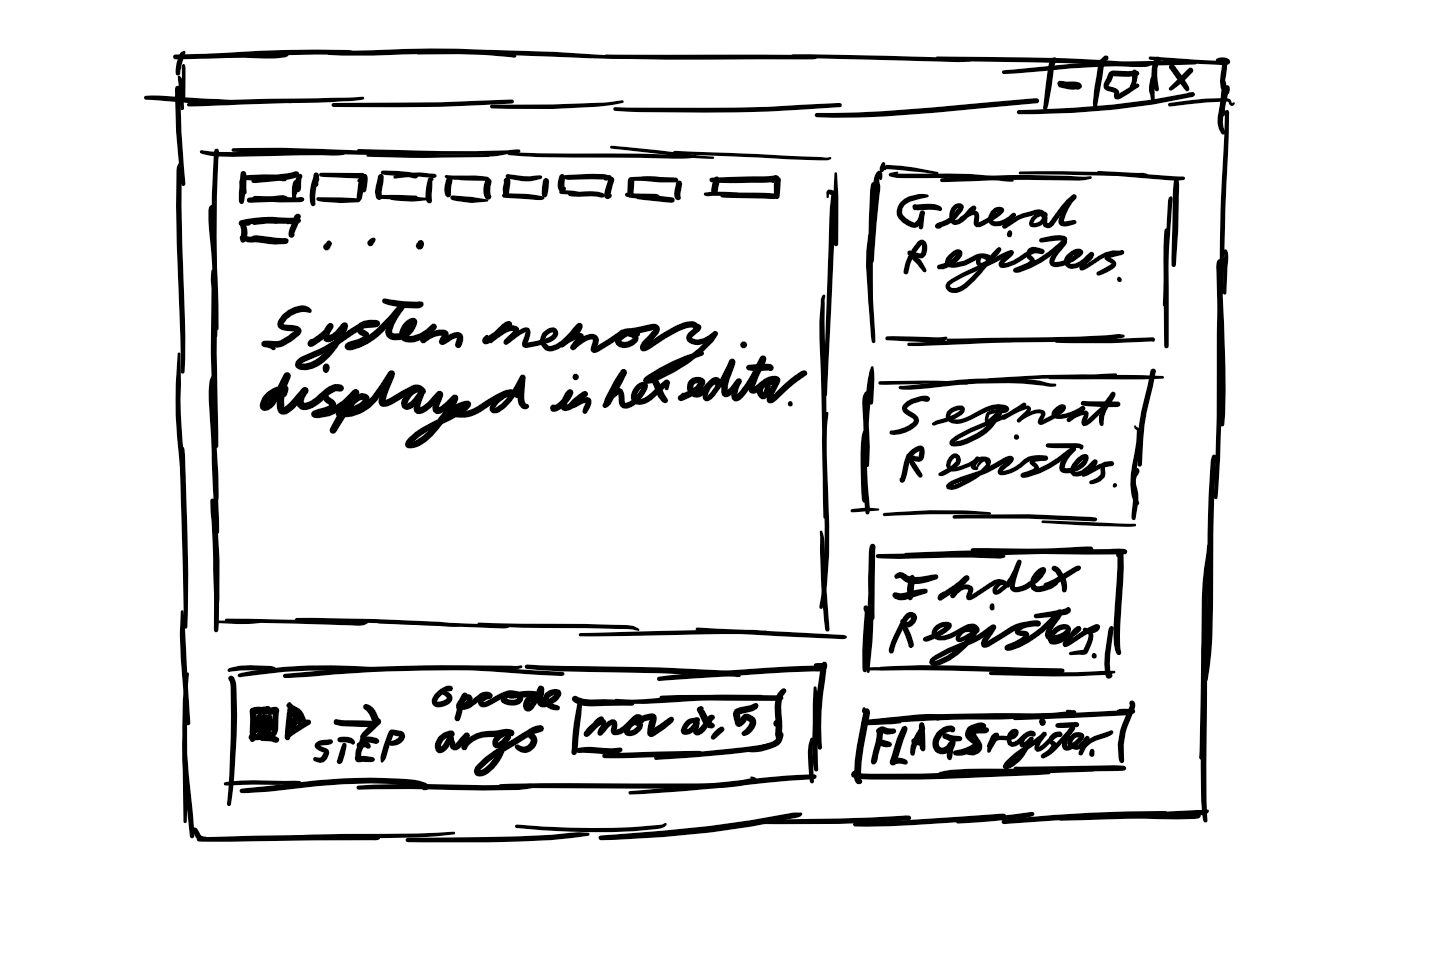
\includegraphics[scale=0.4]{gui-first-design}
        \caption{Initial GUI design drawn on a Surface Pro tablet.}
        \label{figure:gui-first-design}
    \end{figure}

    The hex editor would display and allow the user to alter system memory, the status/control panel would show the disassembled instruction currently being run and will the user to play/pause execution as well as change execution speed, while finally the register panels will each display and will allow for the editing of the values of all the different register groups (general-purpose, segments, index registers, stack registers and FLAGS register).